% !TEX TS-program = XeLaTeX
% use the following command: 
% all document files must be coded in UTF-8
\documentclass{textolivre}
% for anonymous submission
%\documentclass[anonymous]{textolivre}
% to create HTML use 
%\documentclass{textolivre-html}
% See more information on the repository: https://github.com/leolca/textolivre

% Metadata
\begin{filecontents*}[overwrite]{article.xmpdata}
    \Title{Principais vertentes dos estudos do letramento no Brasil}
    \Author{Cícero da Silva \sep Adair Vieira Gonçalves}
    \Language{pt}
    \Keywords{Estudos do letramento \sep Ensino-aprendizagem \sep Pesquisa \sep Brasil \sep Novos Estudos do Letramento.}
    \Journaltitle{Texto Livre}
    \Journalnumber{1983-3652}
    \Volume{14}
    \Issue{1}
    \Firstpage{1}
    \Lastpage{16}
    \Doi{10.35699/1983-3652.2021.29164}

    \setRGBcolorprofile{sRGB_IEC61966-2-1_black_scaled.icc}
            {sRGB_IEC61966-2-1_black_scaled}
            {sRGB IEC61966 v2.1 with black scaling}
            {http://www.color.org}
\end{filecontents*}

% used to create dummy text for the template file
\definecolor{dark-gray}{gray}{0.35} % color used to display dummy texts
\usepackage{lipsum}
\SetLipsumParListSurrounders{\colorlet{oldcolor}{.}\color{dark-gray}}{\color{oldcolor}}

% used here only to provide the XeLaTeX and BibTeX logos
\usepackage{hologo}

% used in this example to provide source code environment
%\crefname{lstlisting}{lista}{listas}
%\Crefname{lstlisting}{Lista}{Listas}
%\usepackage{listings}
%\renewcommand\lstlistingname{Lista}
%\lstset{language=bash,
        breaklines=true,
        basicstyle=\linespread{1}\small\ttfamily,
        numbers=none,xleftmargin=0.5cm,
        frame=none,
        framexleftmargin=0.5em,
        framexrightmargin=0.5em,
        showstringspaces=false,
        upquote=true,
        commentstyle=\color{gray},
        literate=%
           {á}{{\'a}}1 {é}{{\'e}}1 {í}{{\'i}}1 {ó}{{\'o}}1 {ú}{{\'u}}1 
           {à}{{\`a}}1 {è}{{\`e}}1 {ì}{{\`i}}1 {ò}{{\`o}}1 {ù}{{\`u}}1
           {ã}{{\~a}}1 {ẽ}{{\~e}}1 {ĩ}{{\~i}}1 {õ}{{\~o}}1 {ũ}{{\~u}}1
           {â}{{\^a}}1 {ê}{{\^e}}1 {î}{{\^i}}1 {ô}{{\^o}}1 {û}{{\^u}}1
           {ä}{{\"a}}1 {ë}{{\"e}}1 {ï}{{\"i}}1 {ö}{{\"o}}1 {ü}{{\"u}}1
           {Á}{{\'A}}1 {É}{{\'E}}1 {Í}{{\'I}}1 {Ó}{{\'O}}1 {Ú}{{\'U}}1
           {À}{{\`A}}1 {È}{{\`E}}1 {Ì}{{\`I}}1 {Ò}{{\`O}}1 {Ù}{{\`U}}1
           {Ã}{{\~A}}1 {Ẽ}{{\~E}}1 {Ũ}{{\~u}}1 {Õ}{{\~O}}1 {Ũ}{{\~U}}1
           {Â}{{\^A}}1 {Ê}{{\^E}}1 {Î}{{\^I}}1 {Ô}{{\^O}}1 {Û}{{\^U}}1
           {Ä}{{\"A}}1 {Ë}{{\"E}}1 {Ï}{{\"I}}1 {Ö}{{\"O}}1 {Ü}{{\"U}}1
           {ç}{{\c{c}}}1 {Ç}{{\c{C}}}1
}


\journalname{Texto Livre: Linguagem e Tecnologia}
\thevolume{14}
\thenumber{1}
\theyear{2021}
\receiveddate{\DTMdisplaydate{2021}{1}{25}{-1}} % YYYY MM DD
\accepteddate{\DTMdisplaydate{2021}{3}{1}{-1}}
\publisheddate{\DTMdisplaydate{2021}{4}{5}{-1}}
% Corresponding author
\corrauthor{Cícero da Silva}
% DOI
\articledoi{10.35699/1983-3652.2021.29164}
% list of available sesscions in the journal: articles, dossier, reports, essays, reviews, interviews, editorial
\articlesessionname{Linguística e Tecnologia}
% Abbreviated author list for the running footer
\runningauthor{Silva e Gonçalves}
\editorname{Daniervelin Pereira}

\title{Principais vertentes dos estudos do letramento no Brasil}
\othertitle{Principales vertientes de los estudios de alfabetización en Brasil}
\othertitle{Main directions of literacy studies in Brazil}
% if there is a third language title, add here:
%\othertitle{Artikelvorlage zur Einreichung beim Texto Livre Journal}

%Não estão aparecendo todos os títulos!

\author[1]{Cícero da Silva \orcid{0000-0001-6071-6711} \thanks{Email: \url{cicolinas@yahoo.com.br}}}
\author[2]{Adair Vieira Gonçalves \orcid{0000-0003-4998-9692} \thanks{Email: \url{adairgoncalves@uol.com.br}}}

\affil[1]{Universidade Federal do Tocantins, Palmas, TO, Brasil.}
\affil[2]{Universidade Federal da Grande Dourados, Dourados, MS, Brasil.}

\addbibresource{article.bib}
% use biber instead of bibtex
% $ biber tl-article-template

% set language of the article
\setdefaultlanguage{portuguese}
\setotherlanguage{spanish}
\setotherlanguage{english}

% for spanish, use:
%\setdefaultlanguage{spanish}
%\gappto\captionsspanish{\renewcommand{\tablename}{Tabla}} % use 'Tabla' instead of 'Cuadro'

% for languages that use special fonts, you must provide the typeface that will be used
% \setotherlanguage{arabic}
% \newfontfamily\arabicfont[Script=Arabic]{Amiri}
% \newfontfamily\arabicfontsf[Script=Arabic]{Amiri}
% \newfontfamily\arabicfonttt[Script=Arabic]{Amiri}
%
% in the article, to add arabic text use: \textlang{arabic}{ ... }

\usepackage{tablefootnote}

\begin{document}
\maketitle

\begin{polyabstract}
\begin{abstract}
Neste artigo, objetiva-se contextualizar as vertentes dos estudos do letramento no Brasil, pontuando as principais linhas de investigação e referencial teórico. A pesquisa é de natureza bibliográfica, de abordagem qualitativo-interpretativista. Primeiramente, buscou-se na literatura referências que tratam de estudos do(s) letramento(s) e que se vinculam a diferentes linhas de pesquisa, como letramento acadêmico, letramento escolar, letramento do professor, letramento digital, letramento literário e letramento científico. Em seguida, realizou-se uma Consulta Parametrizada no sítio do Diretório dos Grupos de Pesquisa no Brasil do Conselho Nacional de Desenvolvimento Científico e Tecnológico para identificar as linhas de pesquisa e seus respectivos grupos de pesquisa vinculados aos estudos do(s) letramento(s) no Brasil. O estudo revelou que já existem bastantes referências acerca do tema no país e as perspectivas de investigação dos letramentos reforçam a importância e contribuições das pesquisas originárias no Grupo Nova Londres, alicerçadas pelos Novos Estudos do Letramento.

\keywords{Estudos do letramento \sep Ensino-aprendizagem \sep Pesquisa \sep Brasil \sep Novos Estudos do Letramento}
\end{abstract}

\begin{spanish}
\begin{abstract}
El objetivo de este artículo es contextualizar los estudios de alfabetización en Brasil, puntualizando las líneas de investigación y marcos teóricos principales. Esta exploración es de naturaleza bibliográfica, con un enfoque cualitativo-interpretativo. Primero, se plantean las referencias sobre los estudios de alfabetización y sus diferentes líneas, como la alfabetización académica, la escolar, la docente, la digital, la literaria y la científica. Luego, se realiza una consulta parametrizada en el sitio web del Directorio de Grupos de Investigación en Brasil, perteneciente al Consejo Nacional para el Desarrollo Científico y Tecnológico, donde se identifican las líneas y respectivos grupos investigativos vinculados a los estudios de alfabetización. Este levantamiento revela suficientes referencias sobre el tema, así como que las diversas perspectivas corroboran la trascendencia y las contribuciones de estas líneas investigativas, promovidas por el New London Group y los Nuevos Estudios de Alfabetización.

\keywords{Estudios de alfabetización \sep Enseñanza-aprendizaje \sep Investigación \sep Brasil \sep Nuevos Estudios de Alfabetización}
\end{abstract}
\end{spanish}

\begin{english}
\begin{abstract}
In this paper, we contextualize the literacy studies in Brazil, providing the main lines of research and theoretical frameworks. The study is bibliographical with a qualitative-interpretative approach. First, we searched the literature for references related to literacy studies and the links to different research lines, such as academic literacy, school literacy, teacher’s literacy, digital literacy, literary literacy, and scientific literacy. Then, a parameterized consult was carried out on the website of the Directory of Research Groups in Brazil, from the National Council for Scientific and Technological Development, to identify the lines of research and their respective research groups related to literacy studies in Brazil. The study revealed that there are enough references on the subject and the prospects for literacy research reinforce the importance and contributions of the research originated in the New London Group and the New Literacy Studies.

\keywords{Literacy studies \sep Teaching-learning \sep Research \sep Brazil \sep New Literacy Studies}
\end{abstract}
\end{english}

% if there is another abstract, insert it here using the same scheme
\end{polyabstract}


\section{Palavras iniciais}\label{sec-intro}
O tema \textit{letramento}, pelas dimensões que alcançou nas duas últimas décadas no meio acadêmico brasileiro, aparece em estudos que se vinculam a diferentes linhas de pesquisa, como letramento acadêmico, letramento escolar, letramento do professor, letramento digital, letramento literário, letramento científico, entre outras. Na mesma medida, também cresceu o número de trabalhos acadêmicos produzidos a respeito do letramento no país, seja em forma de dissertações, teses, artigos e livros. Do mesmo modo, as pesquisas desenvolvidas são caracterizadas por diferentes perspectivas e metodologias, conforme o panorama apresentado neste artigo.

Para corroborar a existência dessas linhas de pesquisa, além da leitura de obras de autores renomados em estudos do letramento no Brasil, realizamos no ano de 2020 uma Consulta Parametrizada no sítio do Diretório dos Grupos de Pesquisa no Brasil (DGPB) do Conselho Nacional de Desenvolvimento Científico e Tecnológico (CNPq) para identificar as linhas de pesquisa (e seus respectivos grupos de pesquisa) digitando palavras-chave como: \textit{letramento acadêmico, letramento escolar, letramento do professor, letramento digital, letramento literário e letramento científico}. Os resultados mostraram que nessa data existiam cadastrados (em diferentes grupos de pesquisa vinculados a instituições de ensino e pesquisa brasileiras de diferentes regiões do país) no Diretório dos Grupos de Pesquisa no Brasil do CNPq, respectivamente, \textit{13} linhas de pesquisa em letramento acadêmico, \textit{06 em letramento escolar, 03 em letramento do professor, 20 em letramento digital, 18 em letramento literário e 02 em letramento científico}. Curiosamente, os números mostram que há uma quantidade expressiva de linhas de letramento digital e literário, enquanto em letramento do professor há apenas 03. 

Portanto, todas essas linhas de estudos do letramento têm alguma relação com o escopo de investigação de nossas pesquisas \cite{goncalves_nas_2011, goncalves_interacao_2013, silva_pedagogia_2018, silva_formacao_2019, silva_plano_2020, santos_letramento_2020}. Cabe-nos ainda informar ao leitor que todos esses tipos de letramento se apresentam imbricados e se transformam. Por isso, a nossa opção por delineá-los separadamente é apenas didática.

\section{Procedimentos metodológicos}\label{sec-metodologia}
Considerando o objetivo do estudo e a natureza dos dados, assumimos os procedimentos metodológicos da pesquisa bibliográfica, de abordagem qualitativo-interpretativista. Segundo \textcite[p. 9]{flick_introduco_2009}, “[...] a pesquisa qualitativa está baseada em texto e na escrita, desde notas de campo a transcrições até descrições e interpretações, e, finalmente, à interpretação dos resultados e da pesquisa como um todo”. Esse tipo de pesquisa contribui sobremodo para a interpretação dos dados analisados, sendo que se pode indagar e refletir sobre a temática a partir dos dados levantados de forma diversificada.

Além disso, este trabalho se caracteriza como uma pesquisa bibliográfica, sendo esta caracterizada como “a revisão da literatura sobre as principais teorias que norteiam o trabalho científico. Essa revisão é o que chamamos de levantamento bibliográfico ou revisão bibliográfica, a qual pode ser realizada em livros, periódicos, artigo de jornais, sites da Internet entre outras fontes” \cite[p. 54]{pizzani_arte_2012}. Assim, no intuito de contextualizar as vertentes dos estudos do letramento no Brasil, primeiramente realizou-se uma pesquisa bibliográfica, um componente imprescindível para situar pesquisas já desenvolvidas sobre o tema da investigação. Em nosso estudo, identificamos e analisamos produções acadêmicas como livros, capítulos e artigos sobre o tema focalizado. 

A revisão bibliográfica permite ao pesquisador trazer definições do quadro conceitual relacionado ao tema focalizado na investigação, dando sustentação às análises tecidas com base nos dados de um estudo. Para tanto, primeiramente buscou-se na literatura referências que tratam de estudos do(s) letramento(s) e que se vinculam às diferentes linhas de pesquisa, como letramento acadêmico, letramento escolar, letramento do professor, letramento digital, letramento literário e letramento científico.

Em seguida, realizou-se uma consulta parametrizada em 17 de maio de 2020 no sítio do Diretório dos Grupos de Pesquisa no Brasil (DGPB) do Conselho Nacional de Desenvolvimento Científico e Tecnológico (CNPq) para identificar as linhas de pesquisa, seus respetivos grupos de pesquisa e instituições de ensino e pesquisa vinculados aos estudos do(s) letramento(s) no Brasil. A consulta parametrizada no DGPB/CNPq sobre letramento seguiu os seguintes parâmetros ou configurações de busca: (1) Consultar “base corrente”; (2) Censo: “ATUAL”; (3) Termo de busca: “letramento digital”, por exemplo, em “todas as palavras”; (4) Consultar por: “linha de pesquisa”; (5) Aplicar a busca nos campos: “Nome da linha de pesquisa”; (6) Situação do grupo: “Certificado”/“Não-atualizado”. Os dados da pesquisa foram compilados e ilustrados em tabela e gráficos.

\section{Letramento acadêmico, escolar, do professor, digital, literário e científico}\label{sec-alfabetizacion}
Estamos compreendendo letramento pelo “estado ou condição de quem não apenas sabe ler e escrever, mas cultiva e exerce as práticas sociais que usam a escrita” \cite[p. 47]{soares_escolarizacao_1999}.  É a partir dessa definição inicial que depois no Brasil foram surgindo os vários desdobramentos dos estudos do letramento.


\subsection{Letramento acadêmico}\label{sec-fmt-academica}
Partimos da asserção comprovada em várias pesquisas de que os gêneros acadêmicos não constituem conteúdos nas escolas brasileiras de Ensino Fundamental e Médio. Desse modo, é importante destacar que o desenvolvimento do letramento acadêmico poderia ser realizado, em certo grau e a depender das circunstâncias, no Ensino Médio, com a didatização de gêneros da esfera acadêmica, levando-se em consideração as relações intergenéricas \cite{correa_relacoes_2006} transitando por outros gêneros, tais como a resenha, o resumo, fichamentos, pré-projetos de pesquisa, etc.

Ao analisar as perspectivas teóricas e práticas relacionadas aos “letramentos acadêmicos”, Lea e Street (2014) ressaltam que os estudos pioneiros envolvendo leitura e escrita vinculados a esse modelo de letramento limitavam-se ao ensino superior, embora tal conceito também possa ser aplicado desde os anos iniciais do Ensino Fundamental até o Ensino Médio. As práticas de leitura e de escrita, nesse ponto de vista, são “práticas sociais que variam segundo contexto, cultura e gênero” \cite[p. 477]{komesu_o_2014}. Apesar da existência de variação em tais práticas, depreendemos que o letramento acadêmico envolve princípios pedagógicos, metodológicos e formativos, além de interação, semelhantes em qualquer ambiente educacional. Ademais, os gêneros discursivos que medeiam a leitura e a escrita em sala de aula e os modos de recepção de tais gêneros exigem diálogo e partilha de saberes (locais ou não) entre os atores sociais na produção de sentido.

Apesar da existência da premissa defendida por \textcite{komesu_o_2014} e também por outros pesquisadores (não brasileiros) de que o letramento acadêmico engloba todos os níveis de ensino (básico e superior), na prática, pesquisas no Brasil envolvendo usos da leitura, da escrita e suas tecnologias associados às teorias do letramento enquanto prática social no ambiente de ensino (escola ou universidade) são vinculadas ao chamado “letramento acadêmico” ou ao “letramento escolar”. Neste último, enquadram as pesquisas desenvolvidas no Ensino Básico, a exemplo dos estudos de \textcite{silva_pedagogia_2018, silva_plano_2020}.

Os pressupostos teóricos que ancoram as investigações e metodologias vinculadas à linha de pesquisa letramento acadêmico articulam práticas de leitura e de escrita tanto de docentes quanto de discentes. Nesse sentido, o letramento acadêmico estaria ligado, de alguma maneira, a atividades envolvendo gêneros discursivos específicos e que circulam na academia. Em diálogo com \textcite{lillis_student_2003}, \textcite[p. 37]{fiad_letramentos_2014} asseveram que é preciso destacar as relações dialógicas e de poder estabelecidas entre “professor-aluno, professor-professor, aluno-aluno, professor-aluno-instituição, professor-aluno-comunidade científica, aluno-futura prática docente, professor-aluno-TDIC\footnote{Tecnologias Digitais de Informação e Comunicação (TDIC).}, professor-aluno-sociedade” nas práticas universitárias. Em outras palavras, não se deve estudar os gêneros isoladamente, mas sim vinculados às relações discursivas \cite{lillis_student_2003} e de poder que eles estabelecem nas relações sociais.

Além disso, \textcite[p. 76]{zavala_quem_2010} ressalta que “[...] produzir um texto acadêmico é como cantar uma música com um coro atrás. [...] O acadêmico não pode cantar sozinho porque as outras vozes devem prover uma evidência para o que está cantando”. Compreender e aceitar tal condição significa que existe harmonia (entre formador-aprendiz) na construção do conhecimento. E os estudantes precisam ter consciência de que na produção de textos (não só acadêmicos) ocorrem idas e voltas, ou seja, escrita, leitura, intervenções e reescrita. Tudo em sincronia entre aluno-professor.

Como mostram algumas pesquisas, em sua maioria, as produções textuais (individuais e/ou colaborativas) representadas pelos mais variados gêneros discursivos\footnote{A título de exemplificação, podemos citar os gêneros \textit{redação de vestibular, resumo acadêmico, resenha, relatório de estágio supervisionado, seminário, monografia e artigo científico}.} geradas em sala de aula da esfera universitária ocupam lugar de destaque como objeto de pesquisa e de ensino sob o viés do letramento acadêmico no Brasil. Os trabalhos de \textcite{marinho_escrita_2010, araujo_2013, fiad_letramentos_2014, santos_letramento_2020}, por exemplo, são pesquisas que se filiam a essa vertente. Nesses estudos, os autores concebem percursos de investigação e análise de dados com ênfase no letramento ideológico \cite{street_literacy_1984, street_letramentos_2014}, sendo boa parte das pesquisas caracterizadas como etnográficas.

\subsection{Letramento escolar}\label{sec-escolar}
No Brasil, pesquisas que se filiam a essa linha abordam variadas temáticas, como: usos e práticas de leitura e de escrita na escola (ou fora dela); práticas de leitura/escrita e gerenciamento escolar do uso de espaços extraclasse, como a biblioteca e a sala de informática; relação oral/escrito e letramento nas produções textuais; formação inicial, saberes docentes e implicações no ensino de língua materna; metodologias e suas implicações no ensino de leitura/escrita orientada por gêneros de outras esferas, como a jornalística, entre outras. Nessa perspectiva, estamos compreendendo letramento escolar como um

\begin{quote}
   [...] emaranhado de ações individuais e de grupo, fundamentalmente vinculadas a aparatos institucionais de diversos tipos, desde o mobiliário e aparelhos de apoio, até regimentos internos e programas de ensino, e não um conjunto de conteúdos e metodologias que se vão alterando ou substituindo em função de demandas oficiais e/ou do acesso a novidades acadêmicas. \cite[p. 323]{signorini_letramento_2007}.
\end{quote}

\textcite{rojo_concepcoes_1995, rojo_letramento_2001, signorini_letramento_2007, bunzen_os_2010} seriam pesquisadores representantes da vertente denominada letramento escolar. Signorini (2007) e Rojo (2001), principalmente, focalizam em suas pesquisas embates envolvendo relações dos sujeitos com práticas escolarizadas\footnote{Embora não seja o foco do nosso estudo, com base em \textcite{rojo_letramento_2001} podemos afirmar que uma prática escolar refere-se àquilo que é típico da escola, como é o caso da produção/leitura do gênero redação de vestibular. Já uma prática escolarizada diz respeito aquilo que é inserido na sala de aula como objeto de didatização, neste caso, podemos exemplificar a leitura e a escrita do gênero \textit{artigo de opinião}, que é um gênero próprio da esfera jornalística, mas que tem sido utilizado, com frequência, no contexto escolar.} de leitura e escrita.

A afirmação do letramento escolar como o “modelo” em que também se inscrevem os processos de ensino e aprendizagem da leitura e da escrita na escola (ou fora dela) é sustentada pelas ações de professores e do grupo de atores (gestores, coordenadores das escolas) envolvidos nas práticas educativas. Essa perspectiva compreende o ensino de língua materna como práticas letradas específicas, mas “[...] que estão em relação solidária e/ou de confronto com outras práticas sociais dentro e fora da instituição” \cite[p. 323]{signorini_letramento_2007}. Em outros termos, significa dizer que as práticas de leitura e de escrita na escola estabelecem relações estreitas com contextos sociais influentes da sociedade, a exemplo das esferas acadêmica e jornalística. Zavala afirma que

\begin{quote}
   [...] o letramento escolar é só uma forma de usar a linguagem como parte de uma prática social que ganhou legitimidade por razões ideológicas que se enquadram em relações de poder. Como consequência, as crianças de contextos minoritários, que aprendem a usar a linguagem de maneiras diferentes daquelas que se ensinam na escola, estão em desvantagem quando devem adquirir o tipo de discurso expositivo e ensaístico que caracteriza o letramento escolar \cite[p. 73]{zavala_quem_2010}.
\end{quote}

Por mais que tenha aceitação ampla e desfrute de maior prestígio social, fica explícito nesse excerto que a legitimação do letramento escolar no contexto educacional muitas vezes não reconhece nem valoriza os saberes dos atores sociais pertencentes a grupos minoritários no sistema formal de ensino. Uma criança que não domina a variedade de prestígio da língua, por exemplo, ao produzir um texto, poderia enfrentar mais dificuldades que outras na escrita. A minimização de tal embate depende diretamente de ações e atitudes sensíveis do professor durante o processo de produção textual. E a principal delas é acompanhar o aluno, valorizá-lo e promover contribuições significativas para que ele desenvolva suas capacidades de leitura e de escrita. As pesquisas desenvolvidas nas escolas a respeito do letramento escolar, por exemplo, em sua maioria abordam práticas de leitura e de escrita mais próximas daquilo que \textcite{street_literacy_1984, street_letramentos_2014} denomina letramento autônomo.

\subsection{Letramento do professor}\label{sec-docente}
As pesquisas em letramento do professor, orientadas por diferentes perspectivas e variadas metodologias, têm crescido significativamente nos últimos anos e ocupado lugar de destaque, em especial, no ambiente de atuação profissional, formação inicial e continuada do professor no Brasil. De acordo com \textcite[p. 21]{kleiman_projetos_2009}, podemos compreender “[...] o letramento do professor não como mero instrumento para realização do trabalho, mas como aspecto constitutivo, identitário de sua função como formador de novos leitores e usuários da língua escrita, ou seja, intrinsecamente ligado a sua atuação profissional”. Dentro das investigações – situadas em contextos particularizados –, ganham enfoque as práticas letradas e identitárias profissionais do professor, formação do professor e letramento, além da política de formação docente e letramento.

O letramento do professor, por apresentar dimensões amplas e que englobam a atuação na sala de aula e formação inicial e continuada desse profissional, tem como principal objetivo criar condições para que o docente melhore suas (auto)representações acerca de sua capacidade profissional, bem como a possibilidade de desenvolvimento autônomo das suas funções no ambiente de trabalho \cite{kleiman_projetos_2009}. Os desdobramentos da atuação do professor, por vezes, podem ser refletidos nas práticas letradas das quais esse agente de letramento desenvolve e participa no seu espaço de trabalho, o que pode fortalecer as práticas didático-pedagógicas conduzidas por esse profissional.

A maior parte das contribuições para o desenvolvimento do letramento do professor vem de pesquisas desenvolvidas no campo aplicado dos estudos da linguagem, como os trabalhos de \textcite{kleiman_processos_2006, kleiman_projetos_2009, oliveira_variacao_2010, kleiman_estudos_2014}, além de outros. Todos esses estudos apresentam um olhar reflexivo e arcabouço teórico que podem contribuir para a formação do professor, suas práticas profissionais, identidade como agente de letramento \cite{kleiman_processos_2006, kleiman_projetos_2009} e ação no ambiente de trabalho.

\subsection{Letramento digital}\label{sec-digital}
A interação pela linguagem envolve, principalmente na contemporaneidade, práticas de leitura e escrita mediadas pelo uso das chamadas Tecnologias Digitais de Informação e Comunicação (TDICs), sendo uma prática bastante comum no ensino superior e pós-graduação em diferentes modalidades de ensino (presencial e à distância) e até na educação básica. Tal realidade torna as TDICs um importante elemento facilitador de interação cultural e representação social nas práticas e eventos de letramento de contextos de formação, o que leva o letramento digital a figurar como uma linha de pesquisa importante e de potencial crescimento no meio acadêmico brasileiro.

O estudo de \textcite{araujo_letramento_2014}, além de discorrer acerca da trajetória do(s) conceito(s) de letramento digital recorrente(s) nas décadas de 1970, 1980, 1990 e na contemporaneidade, também apresenta um panorama das pesquisas desenvolvidas na área, pontuando os estudos mais importantes sobre o assunto e os respectivos métodos assumidos nas investigações.

Ao longo dessas cinco décadas, os eventos de letramento envolvendo práticas de leitura e escrita vinculadas, de alguma maneira, a usos das TDICs e ensino em ambiente virtual, receberam diferentes denominações, como letramento visual, letramento tecnológico, letramento computacional, letramento TDIC, letramento informacional e letramento eletrônico \cite{araujo_letramento_2014}. Portanto, o conceito de letramento digital recebe influência de todas essas expressões.

Com base em \textcite{buzato_desafios_2007}, para quem a expressão letramento digital ganha sentido em função do aspecto transcultural da internet, \textcite[p. 301]{araujo_letramento_2014} compreendem letramento digital “[...] como um amálgama de diversos tipos de letramentos que se entrelaçam e se apoiam para os sujeitos construírem-se e constituírem-se através de suas relações sociais em ambientes virtuais”. Em outros termos, essa concepção contempla os usos sociais promovidos pelas TDICs.

Dentre as pesquisas em que os autores investigam o letramento digital vinculado ao ensino em ambientes virtuais ou ao uso das TDICs como suporte no contexto educacional, podemos citar o trabalho de \textcite{coscarelli__letramento_2011, signorini_letramentos_2012, komesu_letramentos_2013, araujo_letramento_2014, vidotti_de_rezende_o_2016, ribeiro_tecnologia_2016}, entre outros. Nesses estudos, os interesses investigativos recaem sobre o aprendizado via mediação tecnológica, apresentando um elo estreito com o letramento ideológico.

Também no contexto brasileiro, é importante destacarmos alguns trabalhos publicados recentemente cujo enfoque é letramentos digitais, ensino no contexto da pandemia da COVID-19 e desafios para docentes e discentes, como os estudos de \textcite{almeida_letramento_2020, arruda__educacao_2020, carneiro_uso_2020, silva_letramento_2020}. Esse conjunto de pesquisas, além de analisar questões inerentes aos letramentos digitais em função das novas demandas pedagógicas na educação básica e superior advindas com a pandemia, discutem também acesso e uso de tais recursos, além de destacarem experiências e práticas pedagógicas que vêm sendo realizadas mediadas pelas TDICs na educação brasileira.

\subsection{Letramento literário}\label{sec-literaria}
No Brasil, a discussão acerca de aspectos teórico-metodológicos relativos ao letramento literário é, na contemporaneidade, um tema que não pode passar por despercebido em uma pesquisa acadêmica como esta, dada a realidade das práticas de leitura e escrita em diferentes esferas da sociedade envolvendo algum texto literário. Nesse sentido, letramento literário designa parte do letramento como um todo, sendo caracterizado pela inserção dos atores sociais no munda da escrita, por meio de práticas de recepção/produção de diferentes tipos de textos escritos que circulam na sociedade \cite{paulino_letramento_2001}.

Em sua obra, \textcite{cosson_letramento_2009} enfoca processo de letramento inerente aos textos literários, além de propor a formação de uma comunidade de leitores que transcenda os limites da sala de aula e da escola. Depreende-se que o processo de letramento literário é diferente da leitura literária por fruição; ou seja, esta depende daquela. Por isso, ao inserirmos a literatura na sala de aula para fins de ensino

\begin{quote}
    [...] devemos compreender que o letramento literário é uma prática social e, como tal, responsabilidade da escola. A questão a ser enfrentada não é se a escola deve ou não escolarizar a literatura, como bem nos alerta Magda Soares, mas sim como fazer essa escolarização sem descaracterizá-la, sem transformá-la em um simulacro de si mesma que mais nega do que confirma seu poder de humanização \cite[p. 23]{cosson_letramento_2009}. 
\end{quote}

Na perspectiva do letramento literário, não se pode exigir que o aluno apenas leia determinada obra literário e, ao final, faça uma prova ou entregue uma ficha de leitura, uma vez que a leitura é desenvolvida com base nos mecanismos propostos pela escola visando à proficiência da leitura literária. Soares (1999), ao discutir o que denomina escolarização da leitura literária no ensino, sugere alternativas que visam a minimizar o tratamento escolar negativo acerca da literatura, sinalizando certos equívocos e algumas alternativas acessíveis aos professores.

Portanto, dentre as principais pesquisas que focalizam o letramento literário, dada a realidade das práticas de leitura e escrita situadas na escola ou em outras esferas da sociedade envolvendo algum texto literário, destacamos os trabalhos de \textcite{lajolo_leitura_1991, soares_escolarizacao_1999, paulino_letramento_2001, cosson_letramento_2009}, dentre outros. Esses trabalhos proporcionaram importantes contribuições para o desenvolvimento das pesquisas na perspectiva do letramento literário no Brasil.

\subsection{Letramento científico}\label{sec-cientifica}
Conforme apresentado anteriormente neste artigo, particularmente no contexto brasileiro, as diferentes vertentes contemporâneas de estudos do(s) letramento(s) são alinhadas aos mais variados usos da linguagem nas práticas de leitura, escrita e suas tecnologias nas práticas sociais. No bojo dessas práticas sociais de usos da linguagem, o letramento se desponta como um importante objeto de investigação científica, a exemplo do chamado letramento científico \cite{santos_educacao_2007, cunha_alfabetizacao_2017}. 

Nessa perspectiva, a problematização do ensino da linguagem científica em sala de aula, bem como suas implicações no que diz respeita à cultura científica da sociedade, são pontos que demandam uma ampla reflexão. \textcite[p. 479]{santos_educacao_2007} ressalta que

\begin{quote}
    [...] na tradição escolar a alfabetização científica tem sido considerada na acepção do domínio da linguagem científica, enquanto o letramento científico, no sentido do uso da prática social, parece ser um mito distante da prática de sala de aula. Ao empregar o termo letramento, busca-se enfatizar a função social da educação científica contrapondo-se ao restrito significado de alfabetização escolar. 
\end{quote}

Com base nesse excerto, depreende-se que a alfabetização seria o processo mais elementar de domínio da linguagem científica. Por sua vez, o letramento exige tanto o domínio da linguagem científica (escrita) quanto o da prática social, alcançando-se assim a educação científica apetecida em seus diferentes graus nos processos cognitivos e domínios de alto nível \cite{santos_educacao_2007}. Em outros termos, letramento científico é “o processo por meio do qual os estudantes estarão aptos a acessar e produzir conhecimentos científicos mediados pela escrita, de modo que possibilite o olhar e a intervenção consciente e crítica no mundo real” \cite[p. 7]{silva_ciencia_2018}. Assim, o letramento científico é responsável por nos oferecer capacidades de usos da linguagem para transitarmos com desenvoltura nos diferentes eventos do nosso cotidiano vinculados, de algum modo, a certo saber científico.

Atrelado a isso, a educação científica contribui, de alguma maneira, para compreensão do mundo que nos cerca e se torna fundamental para a formação do pensamento crítico dos estudantes em processo de formação, preparando-os como atores sociais capazes de visualizar a importância do letramento científico no desenvolvimento de pesquisas sobre educação em ciências ou em outras áreas.

Por tudo isso, o letramento científico tem ocupado espaço importante em pesquisas brasileiras vinculadas a diferentes áreas com enfoque em educação científica, as quais situam referenciais e tecem reflexões sobre currículo, filosofia, política educacional, escrita acadêmica, formação de professores na tentativa de analisar o papel social da educação científica na formação do cidadão \cite{santos_educacao_2007}. E grande parte das contribuições para o desenvolvimento do letramento científico vem de pesquisas desenvolvidas na área da educação em ciências e estudos da linguagem, como os trabalhos de \textcite{santos_educacao_2007, motta-roth_letramento_2011, cunha_alfabetizacao_2017, silva_ciencia_2018}, dentre outros.

\subsection{Discussão dos dados}\label{sec-discusion}
Para ilustrar os resultados da consulta parametrizada realizada no sítio dos Grupos de Pesquisa no Brasil (DGPB) do \textcite{consejo_nacional_de_desarrollo_cientifico_y_tecnologico__cnpq_directorio_nodate}\footnote{Para maiores detalhes, consultar o sítio do Diretório dos Grupos de Pesquisa no Brasil/CNPq em: \url{http://dgp.cnpq.br/dgp/faces/consulta/consulta_parametrizada.jsf} acesso em: 17 mai. 2020.} a fim de identificar as linhas de pesquisa caracterizas anteriormente, criou-se a \Cref{tbl01}.

\begin{table}[htpb]
\caption{Distribuição das linhas de pesquisa sobre letramento no DGPB/CNPq.}
\label{tbl01}
\begin{tabular}{llll}
\toprule
\textbf{Linha de pesquisa}    & \textbf{Quantidade} & \textbf{\%}    & \textbf{Instituição\tablefootnote{Legenda de siglas das instituições de ensino e pesquisa brasileiras que as linhas e grupos de pesquisa estão vinculados: IFBA - Instituto Federal da Bahia; IFCE - Instituto Federal do Ceará; IF-Farroupilha - Instituto Federal Farroupilha; IFRN - Instituto Federal do Rio Grande do Norte; IFRS - Instituto Federal do Rio Grande do Sul; IFSC - Instituto Federal de Santa Catarina; PUC/PR - Pontifícia Universidade Católica do Paraná; UEM - Universidade Estadual de Maringá; UEMA - Universidade Estadual do Maranhão; UEMASUL - Universidade Estadual da Região Tocantina do Maranhão; UERGS - Universidade Estadual do Rio Grande do Sul; UESPI - Universidade Estadual do Piauí; UERJ - Universidade do Estado do Rio de Janeiro; UESB - Universidade Estadual do Sudoeste da Bahia; UESC - Universidade Estadual de Santa Cruz; UFAL - Universidade Federal de Alagoas; UFBA - Universidade Federal da Bahia; UFERSA - Universidade Federal Rural do Semi-Árido; UEMG - Universidade do Estado de Minas Gerais; UFMG - Universidade Federal de Minas Gerais; UFPA - Universidade Federal do Pará; UFPB - Universidade Federal da Paraíba; UFPE - Universidade Federal de Pernambuco; UFPR - Universidade Federal do Paraná; UFRB - Universidade Federal do Recôncavo da Bahia; UFRN - Universidade Federal do Rio Grande do Norte; UFRPE - Universidade Federal Rural de Pernambuco; UFRR - Universidade Federal de Roraima; UFSCar - Universidade Federal de São Carlos; UFSJ - Universidade Federal de São João Del-Rei; UFSM - Universidade Federal de Santa Maria; UFT - Universidade Federal do Tocantins; UFTM - Universidade Federal do Triângulo Mineiro; UNEB - Universidade do Estado da Bahia; UNESP - Universidade Estadual Paulista Júlio de Mesquita; UNICAMP - Universidade Estadual de Campinas; UNIOESTE - Universidade Estadual do Oeste do Paraná; UNIPAMPA - Universidade Federal do Pampa; UNIR - Universidade Federal de Rondônia; UNITAU - Universidade de Taubaté; UNIVILLE - Universidade da Região de Joinville; USP - Universidade de São Paulo; UTFPR - Universidade Tecnológica Federal do Paraná.}}            \\
\midrule
L1. Letramento acadêmico &
  13 &
  21\% &
  \begin{tabular}[c]{@{}l@{}}IFCE, UNIVILLE, UEM, UFERSA, IFRS, \\ UFT, PUC/PR, UTFPR, UFMG, IFBA, \\ UFRB, UFPR, UFSJ\end{tabular} \\
\midrule
L2. Letramento escolar         & 6                 & 10\%           & USP, UERJ, UEMASUL, UFMG, UFSCar \\
\midrule
L3. Letramento do professor         & 3                 & 5\%            & UFPE, UNITAU, UNICAMP            \\
\midrule
L4. Letramento digital &
  20 &
  32\% &
  \begin{tabular}[c]{@{}l@{}}UEMA, UFPR, UFRPE, UEMG, UFMG, \\ UFRN, UNIPAMPA, UNIVILLE, IFSC, \\ UFERSA, UNITAU, UFSCar, UFSM, \\ UESB, UFBA, UFPB, UTFPR, UNEB, \\ UNESP\end{tabular} \\
\midrule
L5. Letramento literário &
  18 &
  29\% &
  \begin{tabular}[c]{@{}l@{}}UESC, UFRR, UFAL, UFMG, UFTM, UFT, \\ UNIVILLE, UFPE, UFPA, IFRN, UNIR, \\ UNITAU, IF-Farroupilha, UERGS, \\ UNIOESTE\end{tabular} \\
\midrule
L6. Letramento científico      & 2                 & 3\%            & UESPI, IFSC                      \\
\multicolumn{1}{c}{\textbf{Total}} & \textbf{62}       & \textbf{100\%} &  \\
\bottomrule
\end{tabular}
\source{dados da pesquisa (2020).}
\end{table}

%não está aparecendo a nota de rodapé 5, inserida na tabela. Deve ser pq é longa

Os dados da \Cref{tbl01} mostram os seguintes números de linhas de pesquisa sobre letramento registradas no DGPB/CNPq: 13 em L1. Letramento acadêmico; 06 em L2. Letramento escolar; 03 em L3. Letramento do professor; 20 em L4. Letramento digital; 18 em L5. Letramento literário; e 02 em L6. Letramento científico. Ao todo, foi identificado um total de 62 linhas de pesquisa sobre letramento, as quais estão vinculadas a 43 instituições de ensino e pesquisa brasileiras.

\begin{figure}[htbp]
 \centering
 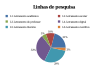
\includegraphics[width=0.95\textwidth]{Fig01_pt.pdf}
 \caption{Participação da L1, L2, L3, L4, L5 e L6 no universo de 62 linhas de pesquisa.}
 \label{fig01}
 \source{dados da pesquisa (2020).}
\end{figure}

%A figura 1 não está aparecendo bem

Considerando-se o total de 62 linhas de pesquisa sobre letramento identificadas no DGPB/CNPq, os números de cada uma das linhas correspondem aos seguintes percentuais: L1, 21\%; L2, 10\%; L3, 5\%; L4, 32\%; L5, 29\%; e L6, 3\%. Esses números ilustrados na \Cref{fig01} sugerem que a L4 e a L5 são predominantes, respectivamente com 32\% e 29\%. No caso da L4, explica-se pelo fato de na contemporaneidade o uso das TDICs na vida cotidiana e em ambientes educacionais seja muito comum. Evidentemente, a utilização das tecnologias digitais mediando diversos meios de comunicação (escrita ou oral) nas práticas sociais gera demandas, sobretudo, para o ensino, o que também está ligado diretamente ao letramento digital. 

Por outro lado, embora a L3 seja fundamental para o desenvolvimento da educação, esta possui apenas 5\% dos registros no DGPB/CNPq. A seguir, apresentamos a \Cref{fig02}, que traz a distribuição das linhas de pesquisa sobre letramento nas diferentes regiões brasileiras.

\begin{figure}[htbp]
 \centering
 \includegraphics[width=0.85\textwidth]{Fig02_pt.png}
 \caption{Distribuição das linhas de pesquisa sobre letramento por região geográfica brasileira segundo o DGPB/CNPq.}
 \label{fig02}
 \source{dados da pesquisa (2020).}
\end{figure}

Conforme ilustrado na \Cref{tbl01}, as 62 linhas de pesquisa sobre letramento (L1, L2, L3, L4, L5 e L6) estão vinculadas a grupos de pesquisa de 43 instituições brasileiras de ensino e pesquisa. Na sequência, com base nos dados da \Cref{tbl01} e da \Cref{fig02}, abordaremos os respectivos números dessas linhas distribuídas por 05 grandes regiões geográficas do Brasil.

\textit{L1. Letramento acadêmico}: os dados da \Cref{tbl01} mostram que a L1 possui um total de 13 linhas registradas em diferentes grupos de pesquisa no DGPB/CNPq. Elas estão vinculadas a 13 instituições ensino e pesquisa diferentes, sendo: IFCE, UNIVILLE, UEM, UFERSA, IFRS, UFT, PUC/PR, UTFPR, UFMG, IFBA, UFRB, UFPR e UFSJ. Considerando a distribuição geográfica, a \Cref{fig02} revela que a L1 possui 01 linha na região Norte, 06 na região Sul, 02 no Sudeste e 04 no Nordeste.

\textit{L2. Letramento escolar}: por sua vez, a L2 possui apenas 06 linhas registradas em diferentes grupos de pesquisa no DGPB/CNPq. A pesquisa mostra que a L2 está vinculada a 05 instituições diferentes, a saber: USP, UERJ, UEMASUL, UFMG e UFSCar. É importante destacar que a UFMG possui dois registros da L2, vinculados a dois grupos de pesquisa diferentes. Segundo os dados da \Cref{fig02}, a L2 está presente em apenas duas regiões brasileiras, sendo 01 linha no Nordeste e 05 no Sudeste.

\textit{L3. Letramento do professor}: na pesquisa, foram encontrados apenas 03 registros da L3 vinculados a 03 grupos de pesquisa diferentes no DGPB/CNPq. A L3 está vinculada a 03 instituições diferentes: UFPE, UNITAU e UNICAMP. A \Cref{fig02} revela que a L3 também está presente em apenas duas regiões: há 01 linha no Nordeste e 02 no Sudeste.

\textit{L4. Letramento digital}: os achados da pesquisa mostram que a L4 possui um total de 20 registros no DGPB/CNPq. Conforme pontuado anteriormente, a L4 possui o maior número de registros e estes estão vinculados a grupos de pesquisa de 19 instituições de ensino e pesquisa diferentes, quais sejam: IFSC, UNIVILLE, UNITAU, UNEB, UEMG, UEMA, UESB, UNESP, UFBA, UFPB, UFMG, UFSM, UFSCar, UNIPAMPA, UFPR, UFRN, UFRPE, UFERSA e UTFPR. Vale ressaltar que a UFERSA possui dois registros da L4, vinculados a dois grupos de pesquisa diferentes. Quanto à distribuição geográfica da L4, ela possui 06 registros na região Sul, 05 no Sudeste e 09 no Nordeste.

\textit{L5. Letramento literário}: a pesquisa revelou que a L5 possui 18 registros no DGPB/CNPq. A L5 é a segunda linha com o maior número de registros e está vinculada a grupos de pesquisa de 15 instituições de ensino e pesquisa diferentes, a saber: UESC, UFRR, UFAL, UFMG, UFTM, UFT, UNIVILLE, UFPE, UFPA, IFRN, UNIR, UNITAU, IF-Farroupilha, UERGS e UNIOESTE. É importante destacar que a UNIR possui 03 registros da L5 e a UFPA possui 02, todos vinculados a grupos de pesquisa diferentes. Ademais, a L5 está distribuída com 07 registros na região Norte, 04 na região Sul, 03 no Sudeste e 04 no Nordeste.

\textit{L6. Letramento científico}: segundo resultados da pesquisa ilustrados na \Cref{tbl01}, a L6 traz apenas 02 registros vinculados a 02 grupos de pesquisa diferentes no DGPB/CNPq. Os grupos de pesquisa a que a L6 pertence vinculam-se respectivamente à UESPI e ao IFSC. Apesar de o letramento científico possuir um número razoável de trabalhos publicados, como artigos, ainda é uma linha de pesquisa pouco presente nos grupos de pesquisa brasileiros. A L6 possui um registro para região Sul e outro para a região Nordeste.

É importante destacar que, conforme os achados da pesquisa, não foi encontrado registro de nenhuma das linhas de pesquisa sobre letramento (L1, L2, L3, L4, L5 e L6) vinculada a instituições de ensino e pesquisa da região Centro-Oeste. No entanto, essa constatação não significa que não exista grupo de pesquisa que investigue a temática letramento nessa região. Mas, a presença de qualquer uma dessas linhas nos grupos de pesquisas das instituições é importante para ampliar e fortalecer os estudos do(s) letramento(s) em âmbito nacional. Outra constatação importante é que, dentre as 05 grandes regiões geográficas brasileiras, apenas a região Nordeste é a única que possui registros das 06 de linhas de pesquisa sobre letramento no DGPB/CNPq.

\section{Conclusões}\label{sec-conclusiones}
Portanto, todas as perspectivas de investigação dos letramentos (acadêmico, escolar, do professor, digital, literário e científico) delineadas anteriormente reforçam a importância e contribuições no contexto brasileiro das pesquisas originárias no Grupo Nova Londres, alicerçadas pelos Novos Estudos do Letramento. Nessa mesma direção, o trabalho de \textcite{terra_letramento_2013} propõe contribuir para uma melhor compreensão do letramento, discutindo os modos como esse fenômeno vem sendo abordado concomitante com os usos da escrita no contexto educacional, no atual momento sócio-histórico, em função da sua natureza, contexto cultural, bem como das suas consequências para a sociedade e indivíduos. Depois de problematizar algumas questões sobre letramento, \textcite[p. 29]{terra_letramento_2013} conclui que a vertente dos Novos Estudos do Letramento “é um caminho profícuo para a (re)definição de um letramento escolar capaz de possibilitar ao aluno chances de aplicar em sua vida extraclasse os conteúdos que ele está aprendendo na escola”. Ou seja, de algum modo o letramento proporcionado nas atividades escolares precisa estar articulado à realidade cotidiana dos estudantes.

Ademais, os resultados da pesquisa realizada sobre o uso das tecnologias digitais de informação e comunicação nas escolas brasileiras no ano de 2019 pelo CGI.br mostram um uso intenso das tecnologias entre os alunos em atividades gerais, como acesso às redes sociais (81\%), envio de mensagens por aplicativos (89\%) e o consumo de vídeos, programas, filmes e séries na Internet (94\%) \cite{comite_gestor_da_internet_no_brasil_resumo_2019}. Todavia, a pesquisa revela que a utilização destes recursos no desenvolvimento de atividades de escolares, sobretudo por meio de ensino remoto, ainda não fazia parte do cotidiano de grande parte dos estudantes. Ao lado disso, 59\% dos professores de escolas públicas urbanas citaram a falta de um curso específico sobre o uso de tecnologias em atividades de ensino-aprendizagem. Já a dificuldade no uso pedagógico desses recursos com os alunos foi citada por 29\% dos professores de escolas particulares. Embora esses números sejam da educação básica, de certo modo vão refletir no ensino superior, além de mostrar que não é só quem trabalha na rede pública de ensino que enfrenta dificuldades em aplicar as TDICs nas atividades didático-pedagógicas, uma demanda ligada aos letramentos digitais no país. 

Assim, somada à falta de domínio ou conhecimento das tecnologias digitais no ensino por alguns professores e alunos, não podemos esquecer que parte dos alunos não possui sequer acesso à internet em banda larga ou 3G/4G, tampouco de boa qualidade, como mostram os dados sobre acesso domiciliar à internet e ensino remoto durante a pandemia da COVID-19 \cite{nascimento_acesso_2020}. Ao lado disso, aparece o letramento digital. Portanto, todas essas constatações reforçam a necessidade do desenvolvimento de pesquisas enfocando ensino, letramentos digitais e uso das TDICs. Como mostram os dados da nossa pesquisa, o grande número (20) de linhas de pesquisa em letramento digital registradas no DGPB/CNPq parece caminhar nessa direção.

\printbibliography\label{sec-bib}

\end{document}
